\newpage
\subsection{Caso d'uso UC12: Gestione proprio profilo utente}
\label{UC12}
\begin{figure}[ht]
	\centering
	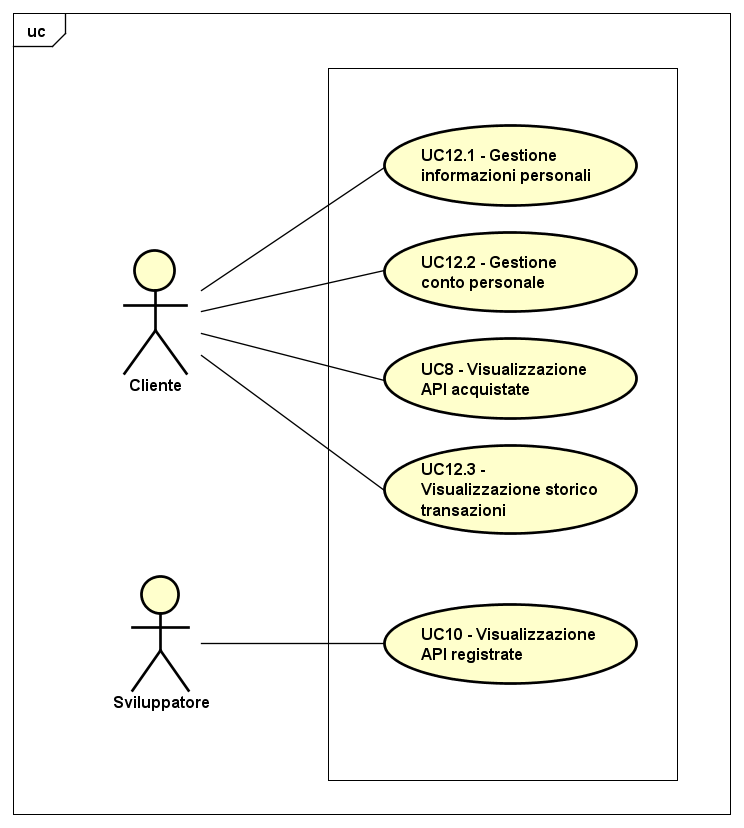
\includegraphics[scale=0.45]{UML/UC12.png}
	\caption{UC12 - Gestione proprio profilo utente}
\end{figure}

\begin{longtable}{ l | p{11cm}}
	\hline
	\rowcolor{Gray}
	\multicolumn{2}{c}{UC12 - Gestione proprio profilo utente} \\
	\hline
	\textbf{Attori} & Cliente, Sviluppatore \\
	\textbf{Descrizione} & L'attore visualizza e/o gestisce le informazioni del proprio profilo utente \\
	\textbf{Pre-Condizioni} & L'attore si trova nella schermata relativa alla gestione del proprio profilo utente \\
	\textbf{Post-Condizioni} & L'attore ha visualizzato e/o gestito le informazioni del proprio profilo utente \\
	\textbf{Scenario Principale} & 
	\begin{enumerate*}[label=(\arabic*.),itemjoin={\newline}]
		\item L'attore può gestire le proprie informazioni personali (UC12.1)
		\item L'attore può gestire il proprio conto utente (UC12.2)
		\item L'attore può visualizzare le API da lui acquistate (UC8)
		\item Lo sviluppatore può visualizzare le API da lui registrate (UC10)
	\end{enumerate*}\\
\end{longtable}

\newpage
\subsubsection{Caso d'uso UC12.1: Gestione informazioni personali}
\label{UC12_1}
\begin{figure}[ht]
	\centering
	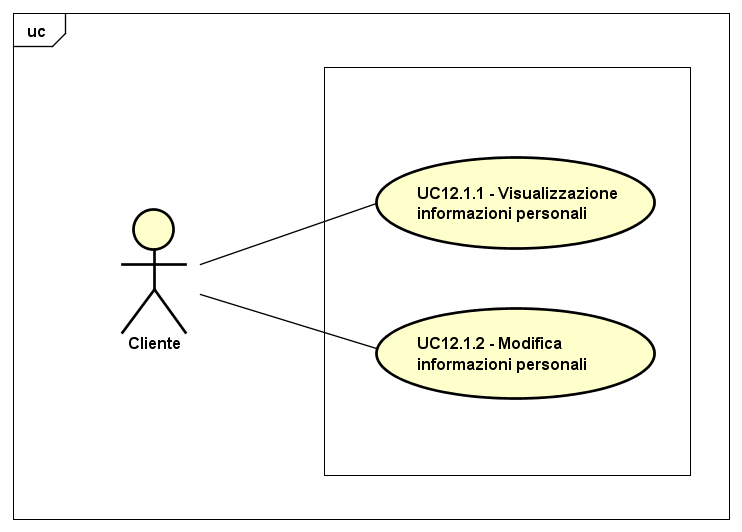
\includegraphics[scale=0.45]{UML/UC12_1.png}
	\caption{UC12.1: Gestione informazioni personali}
\end{figure}

\begin{minipage}{\linewidth}
	\begin{tabular}{ l | p{11cm}}
		\hline
		\rowcolor{Gray}
		\multicolumn{2}{c}{UC12.1 - Gestione informazioni personali} \\
		\hline
		\textbf{Attori} & Cliente \\
		\textbf{Descrizione} & L'attore visualizza e/o modifica le proprie informazioni personali \\
		\textbf{Pre-Condizioni} & L'attore si trova nella schermata relativa alla gestione del proprio profilo utente \\
		\textbf{Post-Condizioni} & L'attore ha visualizzato e/o modificato le proprie informazioni personali \\
		\textbf{Scenario Principale} & 
		\begin{enumerate*}[label=(\arabic*.),itemjoin={\newline}]
			\item L'attore può visualizzare le proprie informazioni personali (UC12.1.1)
			\item L'attore può modificare le proprie informazioni personali (UC12.1.2)
		\end{enumerate*}
	\end{tabular}
\end{minipage}

\newpage
\paragraph{Caso d'uso UC12.1.1: Visualizzazione informazioni personali}
\label{UC12_1_1}
\begin{figure}[ht]
	\centering
	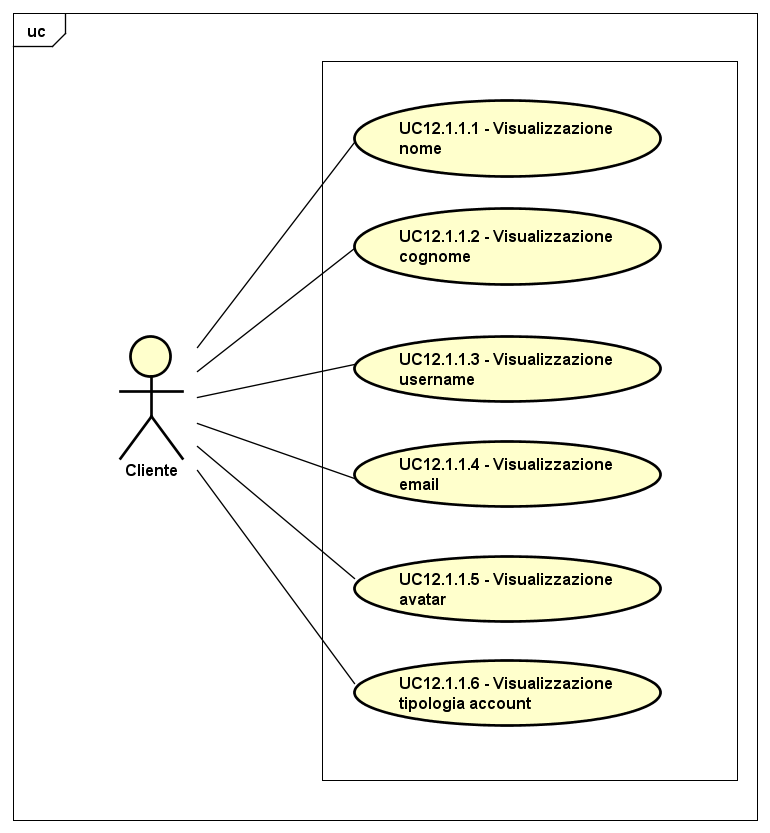
\includegraphics[scale=0.45]{UML/UC12_1_1.png}
	\caption{UC12.1.1: Visualizzazione informazioni personali}
\end{figure}

\begin{minipage}{\linewidth}
\begin{tabular}{ l | p{11cm}}
	\hline
	\rowcolor{Gray}
	\multicolumn{2}{c}{UC12.1.1 - Visualizzazione informazioni personali} \\
	\hline
	\textbf{Attori} & Cliente \\
	\textbf{Descrizione} & L'attore visualizza le proprie informazioni personali \\
	\textbf{Pre-Condizioni} & L'attore si trova nella schermata relativa alla gestione del proprio profilo utente \\
	\textbf{Post-Condizioni} & L'attore ha visualizzato le proprie informazioni personali \\
	\textbf{Scenario Principale} & 
	\begin{enumerate*}[label=(\arabic*.),itemjoin={\newline}]
		\item L'attore può visualizzare il proprio nome (UC12.1.1.1)
		\item L'attore può visualizzare il proprio cognome (UC12.1.1.2)
		\item L'attore può visualizzare il proprio username (UC12.1.1.3)
		\item L'attore può visualizzare la propria email (UC12.1.1.4)
		\item L'attore può visualizzare il proprio avatar (UC12.1.1.5)
		\item L'attore può visualizzare la tipologia del proprio account (UC12.1.1.6)
	\end{enumerate*}\\
\end{tabular}
\end{minipage}

\subparagraph{Caso d'uso UC12.1.1.1: Visualizzazione nome}
\label{UC12_1_1_1}

\begin{minipage}{\linewidth}
\begin{tabular}{ l | p{11cm}}
	\hline
	\rowcolor{Gray}
	\multicolumn{2}{c}{UC12.1.1.1 - Visualizzazione nome} \\
	\hline
	\textbf{Attori} & Cliente \\
	\textbf{Descrizione} & L'attore visualizzare il proprio nome \\
	\textbf{Pre-Condizioni} & L'attore si trova nella schermata relativa alla gestione delle informazioni personali \\
	\textbf{Post-Condizioni} & L'attore ha visualizzato il proprio nome \\
	\textbf{Scenario Principale} & 
	\begin{enumerate*}[label=(\arabic*.),itemjoin={\newline}]
		\item L'attore può visualizzare il proprio nome
	\end{enumerate*}
\end{tabular}
\end{minipage}

\subparagraph{Caso d'uso UC12.1.1.2: Visualizzazione cognome}
\label{UC12_1_1_2}

\begin{minipage}{\linewidth}
	\begin{tabular}{ l | p{11cm}}
		\hline
		\rowcolor{Gray}
		\multicolumn{2}{c}{UC12.1.1.2 - Visualizzazione cognome} \\
		\hline
		\textbf{Attori} & Cliente \\
		\textbf{Descrizione} & L'attore visualizzare il proprio cognome \\
	\textbf{Pre-Condizioni} & L'attore si trova nella schermata relativa alla gestione delle informazioni personali \\
	\textbf{Post-Condizioni} & L'attore ha visualizzato il proprio cognome \\
	\textbf{Scenario Principale} & 
	\begin{enumerate*}[label=(\arabic*.),itemjoin={\newline}]
		\item L'attore può visualizzare il proprio cognome
	\end{enumerate*}
	\end{tabular}
\end{minipage}

\subparagraph{Caso d'uso UC12.1.1.3: Visualizzazione username}
\label{UC12_1_1_3}

\begin{minipage}{\linewidth}
	\begin{tabular}{ l | p{11cm}}
		\hline
		\rowcolor{Gray}
		\multicolumn{2}{c}{UC12.1.1.3 - Visualizzazione username} \\
		\hline
		\textbf{Attori} & Cliente \\
		\textbf{Descrizione} & L'attore visualizzare il proprio username \\
	\textbf{Pre-Condizioni} & L'attore si trova nella schermata relativa alla gestione delle informazioni personali \\
	\textbf{Post-Condizioni} & L'attore ha visualizzato il proprio username \\
	\textbf{Scenario Principale} & 
	\begin{enumerate*}[label=(\arabic*.),itemjoin={\newline}]
		\item L'attore può visualizzare il proprio username
	\end{enumerate*}
	\end{tabular}
\end{minipage}

\subparagraph{Caso d'uso UC12.1.1.4: Visualizzazione email}
\label{UC12_1_1_4}

\begin{minipage}{\linewidth}
	\begin{tabular}{ l | p{11cm}}
		\hline
		\rowcolor{Gray}
		\multicolumn{2}{c}{UC12.1.1.4 - Visualizzazione email} \\
		\hline
		\textbf{Attori} & Cliente \\
		\textbf{Descrizione} & L'attore visualizzare la propria email \\
		\textbf{Pre-Condizioni} & L'attore si trova nella schermata relativa alla gestione delle informazioni personali \\
		\textbf{Post-Condizioni} & L'attore ha visualizzato la propria email \\
		\textbf{Scenario Principale} & 
		\begin{enumerate*}[label=(\arabic*.),itemjoin={\newline}]
			\item L'attore può visualizzare la propria email
		\end{enumerate*}
	\end{tabular}
\end{minipage}

\subparagraph{Caso d'uso UC12.1.1.5: Visualizzazione avatar}
\label{UC12_1_1_5}

\begin{minipage}{\linewidth}
	\begin{tabular}{ l | p{11cm}}
		\hline
		\rowcolor{Gray}
		\multicolumn{2}{c}{UC12.1.1.5 - Visualizzazione avatar} \\
		\hline
		\textbf{Attori} & Cliente \\
		\textbf{Descrizione} & L'attore visualizzare il proprio avatar \\
		\textbf{Pre-Condizioni} & L'attore si trova nella schermata relativa alla gestione delle informazioni personali \\
		\textbf{Post-Condizioni} & L'attore ha visualizzato il proprio avatar \\
		\textbf{Scenario Principale} & 
		\begin{enumerate*}[label=(\arabic*.),itemjoin={\newline}]
			\item L'attore può visualizzare il proprio avatar
		\end{enumerate*}
	\end{tabular}
\end{minipage}

\subparagraph{Caso d'uso UC12.1.1.6: Visualizzazione tipologia account}
\label{UC12_1_1_6}

\begin{minipage}{\linewidth}
	\begin{tabular}{ l | p{11cm}}
		\hline
		\rowcolor{Gray}
		\multicolumn{2}{c}{UC12.1.1.6 - Visualizzazione tipologia account} \\
		\hline
		\textbf{Attori} & Cliente \\
		\textbf{Descrizione} & L'attore visualizzare la tipologia del proprio account \\
		\textbf{Pre-Condizioni} & L'attore si trova nella schermata relativa alla gestione delle informazioni personali \\
		\textbf{Post-Condizioni} & L'attore ha visualizzato la tipologia del proprio account \\
		\textbf{Scenario Principale} & 
		\begin{enumerate*}[label=(\arabic*.),itemjoin={\newline}]
			\item L'attore può visualizzare la tipologia del proprio account
		\end{enumerate*}
	\end{tabular}
\end{minipage}

\newpage
\paragraph{Caso d'uso UC12.1.2: Modifica informazioni personali}
\label{UC12_1_2}
\begin{figure}[ht]
	\centering
	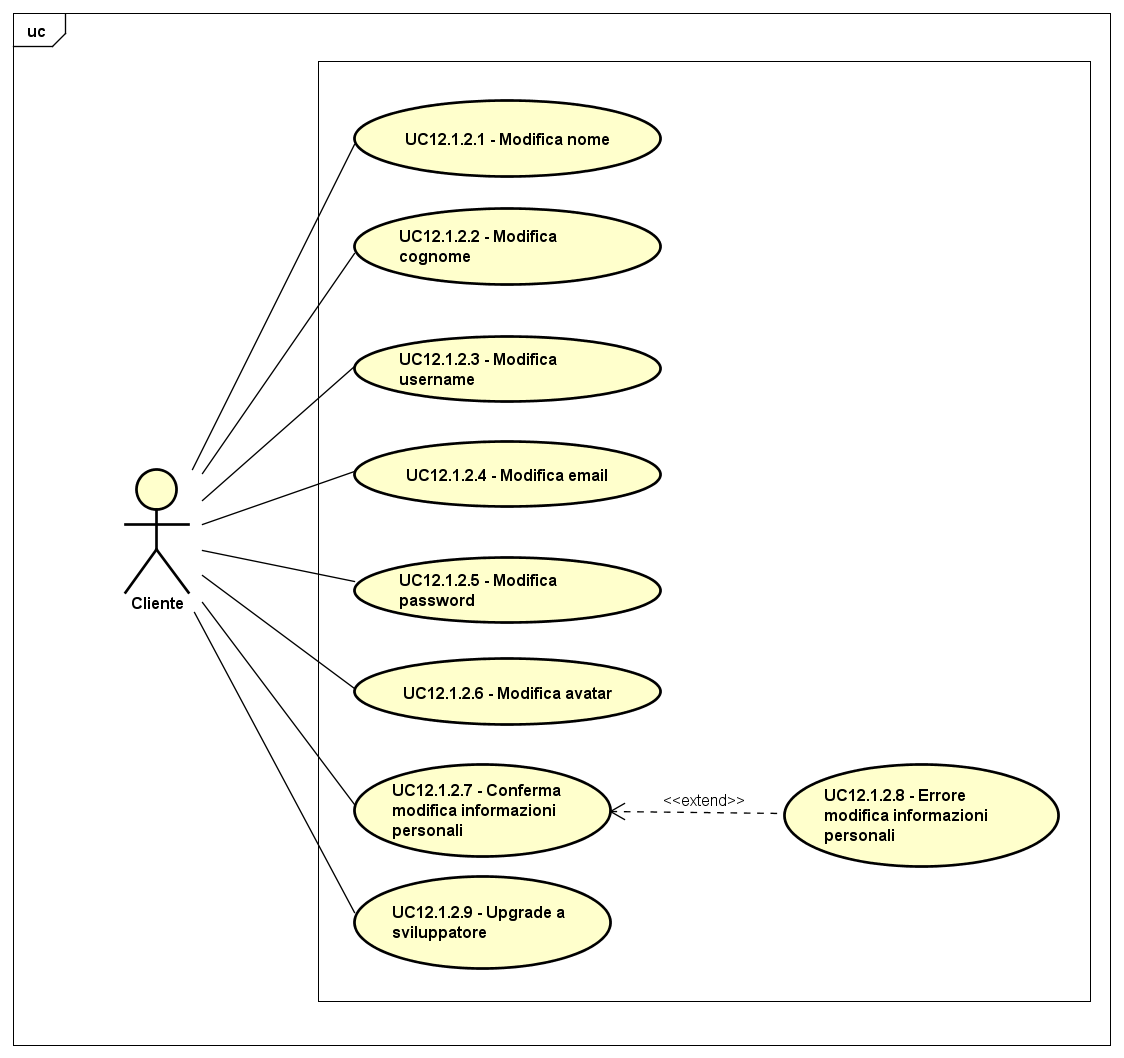
\includegraphics[scale=0.45]{UML/UC12_1_2.png}
	\caption{UC12.1.2: Modifica informazioni personali}
\end{figure}

\begin{tabular}{ l | p{11cm}}
	\hline
	\rowcolor{Gray}
	\multicolumn{2}{c}{UC12.1.2 - Modifica informazioni personali} \\
	\hline
	\textbf{Attori} & Cliente \\
	\textbf{Descrizione} & L'attore modifica le proprie informazioni personali \\
	\textbf{Pre-Condizioni} & L'attore si trova nella schermata relativa alla gestione del proprio profilo utente \\
	\textbf{Post-Condizioni} & L'attore ha modificato le proprie informazioni personali \\
	\textbf{Scenario Principale} & 
	\begin{enumerate*}[label=(\arabic*.),itemjoin={\newline}]
		\item L'attore può modificare il proprio nome (UC12.1.2.1)
		\item L'attore può modificare il proprio cognome (UC12.1.2.2)
		\item L'attore può modificare il proprio username (UC12.1.2.3)
		\item L'attore può modificare la propria email (UC12.1.2.4)
		\item L'attore può modificare la propria password (UC12.1.2.5)
		\item L'attore può modificare il proprio avatar (UC12.1.2.6)
		\item L'attore può confermare la modifica alle proprie informazioni personali (UC12.1.2.7)
	\end{enumerate*}\\
	\textbf{Scenari Alternativi} & 
	\begin{enumerate*}[label=(\arabic*.),itemjoin={\newline}]
		\item L'attore, dopo aver confermato le modifiche alle proprie informazioni personali, può visualizzare un messaggio di errore informativo (E.g: dati non validi, formati dei file errati), e le modifiche non avvengono (UC12.1.2.8)
	\end{enumerate*}\\
\end{tabular}

\subparagraph{Caso d'uso UC12.1.2.1: Modifica nome}
\label{UC12_1_2_1}

\begin{minipage}{\linewidth}
	\begin{tabular}{ l | p{11cm}}
		\hline
		\rowcolor{Gray}
		\multicolumn{2}{c}{UC12.1.2.1 - Modifica nome} \\
		\hline
		\textbf{Attori} & Cliente \\
		\textbf{Descrizione} & L'attore modifica il proprio nome \\
		\textbf{Pre-Condizioni} & L'attore si trova nella schermata relativa alla gestione delle informazioni personali \\
		\textbf{Post-Condizioni} & L'attore ha modificato il proprio nome \\
		\textbf{Scenario Principale} & 
		\begin{enumerate*}[label=(\arabic*.),itemjoin={\newline}]
			\item L'attore può modificare il proprio nome
		\end{enumerate*}
	\end{tabular}
\end{minipage}

\subparagraph{Caso d'uso UC12.1.2.2: Modifica cognome}
\label{UC12_1_2_2}

\begin{minipage}{\linewidth}
	\begin{tabular}{ l | p{11cm}}
		\hline
		\rowcolor{Gray}
		\multicolumn{2}{c}{UC12.1.2.2 - Modifica cognome} \\
		\hline
		\textbf{Attori} & Cliente \\
		\textbf{Descrizione} & L'attore modifica il proprio cognome \\
		\textbf{Pre-Condizioni} & L'attore si trova nella schermata relativa alla gestione delle informazioni personali \\
		\textbf{Post-Condizioni} & L'attore ha modificato il proprio cognome \\
		\textbf{Scenario Principale} & 
		\begin{enumerate*}[label=(\arabic*.),itemjoin={\newline}]
			\item L'attore può modificare il proprio cognome
		\end{enumerate*}
	\end{tabular}
\end{minipage}

\subparagraph{Caso d'uso UC12.1.2.3: Modifica username}
\label{UC12_1_2_3}

\begin{minipage}{\linewidth}
	\begin{tabular}{ l | p{11cm}}
		\hline
		\rowcolor{Gray}
		\multicolumn{2}{c}{UC12.1.2.3 - Modifica username} \\
		\hline
		\textbf{Attori} & Cliente \\
		\textbf{Descrizione} & L'attore modifica il proprio username \\
		\textbf{Pre-Condizioni} & L'attore si trova nella schermata relativa alla gestione delle informazioni personali \\
		\textbf{Post-Condizioni} & L'attore ha modificato il proprio username \\
		\textbf{Scenario Principale} & 
		\begin{enumerate*}[label=(\arabic*.),itemjoin={\newline}]
			\item L'attore può modificare il proprio username
		\end{enumerate*}
	\end{tabular}
\end{minipage}

\subparagraph{Caso d'uso UC12.1.2.4: Modifica email}
\label{UC12_1_2_4}

\begin{minipage}{\linewidth}
	\begin{tabular}{ l | p{11cm}}
		\hline
		\rowcolor{Gray}
		\multicolumn{2}{c}{UC12.1.2.4 - Modifica email} \\
		\hline
		\textbf{Attori} & Cliente \\
		\textbf{Descrizione} & L'attore modifica la propria email \\
		\textbf{Pre-Condizioni} & L'attore si trova nella schermata relativa alla gestione delle informazioni personali \\
		\textbf{Post-Condizioni} & L'attore ha modificato la propria email \\
		\textbf{Scenario Principale} & 
		\begin{enumerate*}[label=(\arabic*.),itemjoin={\newline}]
			\item L'attore può modificare la propria email
		\end{enumerate*}
	\end{tabular}
\end{minipage}

\subparagraph{Caso d'uso UC12.1.2.5: Modifica password}
\label{UC12_1_2_5}

\begin{minipage}{\linewidth}
	\begin{tabular}{ l | p{11cm}}
		\hline
		\rowcolor{Gray}
		\multicolumn{2}{c}{UC12.1.2.5 - Modifica password} \\
		\hline
		\textbf{Attori} & Cliente \\
		\textbf{Descrizione} & L'attore modifica la propria password \\
		\textbf{Pre-Condizioni} & L'attore si trova nella schermata relativa alla gestione delle informazioni personali \\
		\textbf{Post-Condizioni} & L'attore ha modificato la propria password \\
		\textbf{Scenario Principale} & 
		\begin{enumerate*}[label=(\arabic*.),itemjoin={\newline}]
			\item L'attore può modificare la propria password
		\end{enumerate*}
	\end{tabular}
\end{minipage}

\subparagraph{Caso d'uso UC12.1.2.6: Modifica avatar}
\label{UC12_1_2_6}

\begin{minipage}{\linewidth}
	\begin{tabular}{ l | p{11cm}}
		\hline
		\rowcolor{Gray}
		\multicolumn{2}{c}{UC12.1.2.6 - Modifica avatar} \\
		\hline
		\textbf{Attori} & Cliente \\
		\textbf{Descrizione} & L'attore modifica il proprio avatar \\
		\textbf{Pre-Condizioni} & L'attore si trova nella schermata relativa alla gestione delle informazioni personali \\
		\textbf{Post-Condizioni} & L'attore ha modificato il proprio avatar \\
		\textbf{Scenario Principale} & 
		\begin{enumerate*}[label=(\arabic*.),itemjoin={\newline}]
			\item L'attore può modificare il proprio avatar
		\end{enumerate*}
	\end{tabular}
\end{minipage}

\subparagraph{Caso d'uso UC12.1.2.7: Conferma modifica informazioni personali}
\label{UC12_1_2_7}

\begin{minipage}{\linewidth}
	\begin{tabular}{ l | p{11cm}}
		\hline
		\rowcolor{Gray}
		\multicolumn{2}{c}{UC12.1.2.7 - Conferma modifica informazioni personali} \\
		\hline
		\textbf{Attori} & Cliente \\
		\textbf{Descrizione} & L'attore conferma la modifica delle informazioni personali \\
		\textbf{Pre-Condizioni} & L'attore si trova nella schermata relativa alla gestione delle informazioni personali \\
		\textbf{Post-Condizioni} & L'attore ha confermato la modifica delle informazioni personali \\
		\textbf{Scenario Principale} & 
		\begin{enumerate*}[label=(\arabic*.),itemjoin={\newline}]
			\item L'attore può confermare la modifica delle informazioni personali, visualizzando un messaggio di successo
		\end{enumerate*}\\
	\end{tabular}
\end{minipage}

\subparagraph{Caso d'uso UC12.1.2.8: Errore modifica informazioni personali}
\label{UC12_1_2_8}

\begin{minipage}{\linewidth}
	\begin{tabular}{ l | p{11cm}}
		\hline
		\rowcolor{Gray}
		\multicolumn{2}{c}{UC12.1.2.8 - Errore modifica informazioni personali} \\
		\hline
		\textbf{Attori} & Cliente \\
		\textbf{Descrizione} & L'attore visualizza un messaggio di errore informativo e la modifica delle informazioni personali non avviene \\
		\textbf{Pre-Condizioni} & L'attore ha confermato la modifica delle informazioni personali ma si è verificato un errore \\
		\textbf{Post-Condizioni} & L'attore ha visualizzato un messaggio di errore informativo \\
		\textbf{Scenario Principale} & 
		\begin{enumerate*}[label=(\arabic*.),itemjoin={\newline}]
			\item L'attore può visualizzare un messaggio di errore informativo e la modifica delle informazioni personali non avviene
		\end{enumerate*}\\
	\end{tabular}
\end{minipage}

\newpage
\subsubsection{Caso d'uso UC12.2: Gestione conto personale}
\label{UC12_2}
\begin{figure}[ht]
	\centering
	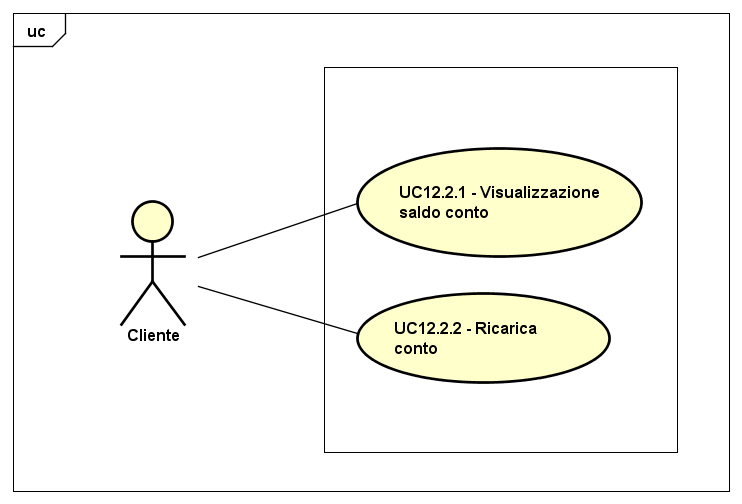
\includegraphics[scale=0.45]{UML/UC12_2.png}
	\caption{UC12.2: Gestione conto personale}
\end{figure}

\begin{minipage}{\linewidth}
	\begin{tabular}{ l | p{11cm}}
		\hline
		\rowcolor{Gray}
		\multicolumn{2}{c}{UC12.2 - Gestione conto personale} \\
		\hline
		\textbf{Attori} & Cliente \\
		\textbf{Descrizione} & L'attore visualizza le informazioni del proprio conto utente e/o effettua una ricarica su di esso \\
		\textbf{Pre-Condizioni} & L'attore si trova nella schermata relativa alla gestione del proprio profilo utente \\
		\textbf{Post-Condizioni} & L'attore ha visualizzato il saldo del proprio conto utente e/o effettuato una ricarica su di esso \\
		\textbf{Scenario Principale} & 
		\begin{enumerate*}[label=(\arabic*.),itemjoin={\newline}]
			\item L'attore può visualizzare il saldo corrente del proprio conto utente (UC12.2.1)
			\item L'attore può effettuare una ricarica sul proprio conto utente (UC12.2.2)
		\end{enumerate*}
	\end{tabular}
\end{minipage}

\paragraph{Caso d'uso UC12.2.1: Visualizzazione saldo conto}
\label{UC12_2_1}

\begin{minipage}{\linewidth}
	\begin{tabular}{ l | p{11cm}}
		\hline
		\rowcolor{Gray}
		\multicolumn{2}{c}{UC12.2.1 - Visualizzazione saldo conto} \\
		\hline
		\textbf{Attori} & Cliente \\
		\textbf{Descrizione} & L'attore visualizza il saldo corrente del proprio conto utente \\
		\textbf{Pre-Condizioni} & L'attore si trova nella schermata relativa alla gestione del proprio conto utente \\
		\textbf{Post-Condizioni} & L'attore ha visualizzato il saldo corrente del proprio conto utente \\
		\textbf{Scenario Principale} & 
		\begin{enumerate*}[label=(\arabic*.),itemjoin={\newline}]
			\item L'attore può visualizzare il saldo corrente del proprio conto utente
		\end{enumerate*}\\
	\end{tabular}
\end{minipage}

\paragraph{Caso d'uso UC12.2.2: Ricarica conto}
\label{UC12_2_2}
\begin{figure}[ht]
	\centering
	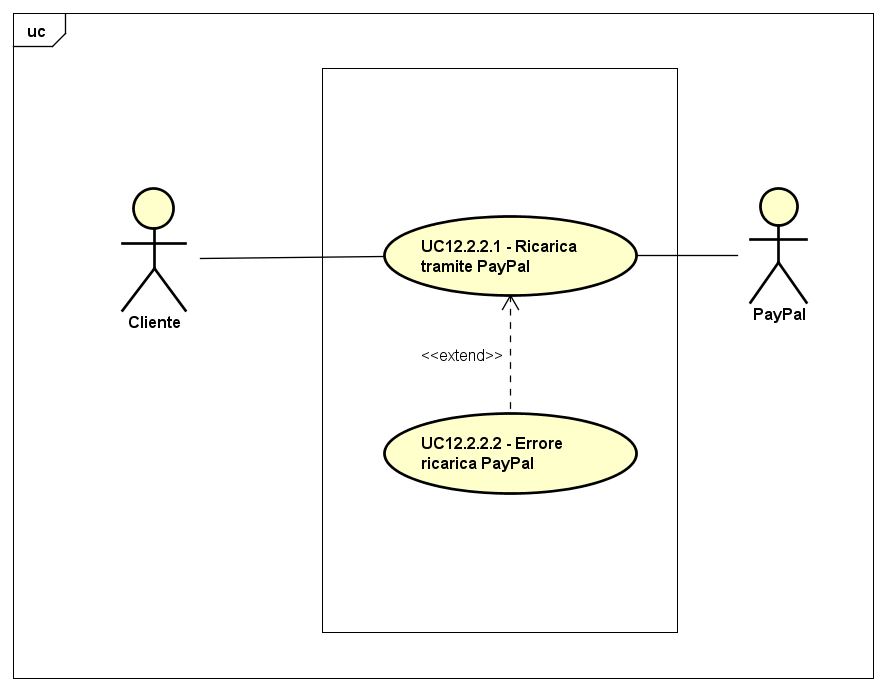
\includegraphics[scale=0.45]{UML/UC12_2_2.png}
	\caption{UC12.2.2: Ricarica conto}
\end{figure}

\begin{minipage}{\linewidth}
	\begin{tabular}{ l | p{11cm}}
		\hline
		\rowcolor{Gray}
		\multicolumn{2}{c}{UC12.2.2 - Ricarica conto} \\
		\hline
		\textbf{Attori} & Cliente, PayPal \\
		\textbf{Descrizione} & L'attore effettua una ricarica sul proprio conto utente \\
		\textbf{Pre-Condizioni} & L'attore si trova nella schermata relativa alla gestione del proprio conto utente \\
		\textbf{Post-Condizioni} & L'attore ha effettuato una ricarica sul proprio conto utente \\
		\textbf{Scenario Principale} & 
		\begin{enumerate*}[label=(\arabic*.),itemjoin={\newline}]
			\item L'attore può effettuare una ricarica tramite PayPal sul proprio conto utente (UC12.2.2.1)
		\end{enumerate*}\\
		\textbf{Scenari Alternativi} & 
		\begin{enumerate*}[label=(\arabic*.),itemjoin={\newline}]
			\item L'attore può visualizzare un messaggio di errore informativo (E.g: dati errati), e la ricarica tramite PayPal sul proprio conto utente non avviene (UC12.2.2.2)
		\end{enumerate*}\\
	\end{tabular}
\end{minipage}

\subparagraph{Caso d'uso UC12.2.2.1: Ricarica tramite PayPal}
\label{UC12_2_2_1}

\begin{minipage}{\linewidth}
	\begin{tabular}{ l | p{11cm}}
		\hline
		\rowcolor{Gray}
		\multicolumn{2}{c}{UC12.2.2.1 - Ricarica tramite PayPal} \\
		\hline
		\textbf{Attori} & Cliente, PayPal \\
		\textbf{Descrizione} & L'attore effettua una ricarica tramite PayPal sul proprio conto utente \\
		\textbf{Pre-Condizioni} & L'attore si trova nella schermata relativa alla ricarica del proprio conto utente \\
		\textbf{Post-Condizioni} & L'attore ha effettuato una ricarica tramite PayPal sul proprio conto utente \\
		\textbf{Scenario Principale} & 
		\begin{enumerate*}[label=(\arabic*.),itemjoin={\newline}]
			\item L'attore può effettuare una ricarica tramite PayPal sul proprio conto utente
		\end{enumerate*}\\
	\end{tabular}
\end{minipage}

\subparagraph{Caso d'uso UC12.2.2.2: Errore ricarica PayPal}
\label{UC12_2_2_2}

\begin{minipage}{\linewidth}
	\begin{tabular}{ l | p{11cm}}
		\hline
		\rowcolor{Gray}
		\multicolumn{2}{c}{UC12.2.2.2 - Errore ricarica PayPal} \\
		\hline
		\textbf{Attori} & Cliente, PayPal \\
		\textbf{Descrizione} & L'attore visualizza un messaggio di errore informativo e la ricarica tramite PayPal sul proprio conto utente non avviene \\
		\textbf{Pre-Condizioni} & L'attore ha confermato la ricarica tramite PayPal sul proprio conto utente ma si è verificato un errore \\
		\textbf{Post-Condizioni} & L'attore ha visualizzato un messaggio di errore informativo \\
		\textbf{Scenario Principale} & 
		\begin{enumerate*}[label=(\arabic*.),itemjoin={\newline}]
			\item L'attore può visualizzare un messaggio di errore informativo e la ricarica tramite PayPal sul proprio conto utente non avviene
		\end{enumerate*}\\
	\end{tabular}
\end{minipage}

\newpage
\subsubsection{Caso d'uso UC12.3: Visualizzazione storico transazioni}
\label{UC12_3}
\begin{figure}[ht]
	\centering
	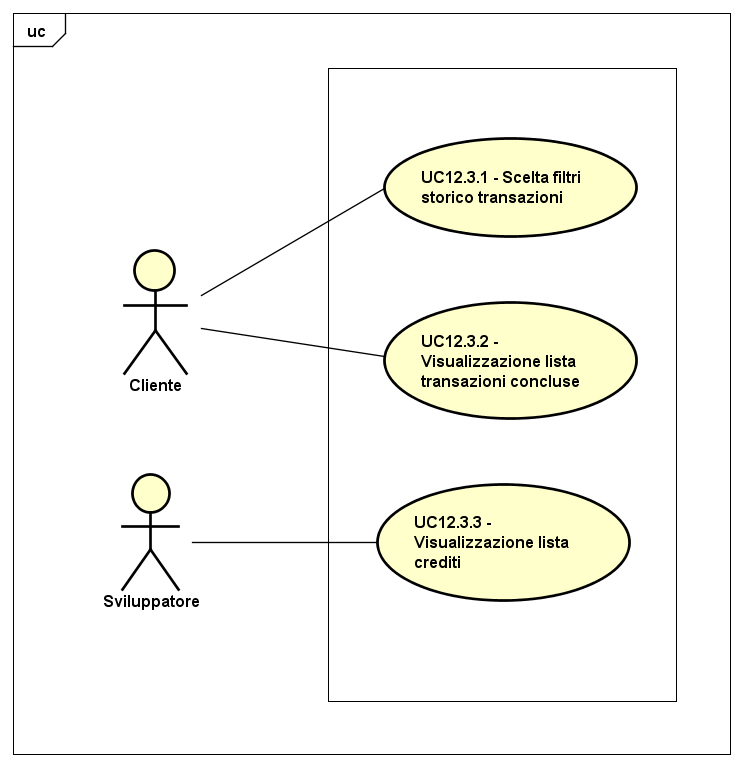
\includegraphics[scale=0.45]{UML/UC12_3.png}
	\caption{UC12.3: Visualizzazione storico transazioni}
\end{figure}

\begin{minipage}{\linewidth}
	\begin{tabular}{ l | p{11cm}}
		\hline
		\rowcolor{Gray}
		\multicolumn{2}{c}{UC12.3 - Visualizzazione storico transazioni} \\
		\hline
		\textbf{Attori} & Cliente, Sviluppatore \\
		\textbf{Descrizione} & L'attore visualizza lo storico delle proprie transazioni \\
		\textbf{Pre-Condizioni} & L'attore si trova nella schermata relativa alla gestione del proprio profilo utente \\
		\textbf{Post-Condizioni} & L'attore ha visualizzato lo storico delle proprie transazioni \\
		\textbf{Scenario Principale} & 
		\begin{enumerate*}[label=(\arabic*.),itemjoin={\newline}]
			\item L'attore può scegliere i filtri di visualizzazione (UC12.3.1)
			\item L'attore può visualizzare la lista delle proprie transazioni concluse (UC12.3.2)
			\item Lo sviluppatore può visualizzare la lista dei propri crediti (UC12.3.3)
		\end{enumerate*}
	\end{tabular}
\end{minipage}

\newpage
\paragraph{Caso d'uso UC12.3.1: Scelta filtri storico transazioni}
\label{UC12_3_1}
\begin{figure}[ht]
	\centering
	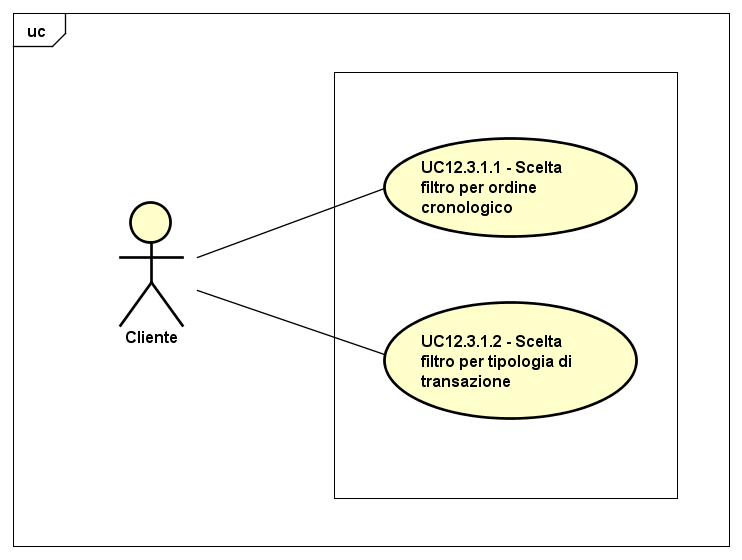
\includegraphics[scale=0.45]{UML/UC12_3_1.png}
	\caption{UC12.3.1: Scelta filtri storico transazioni}
\end{figure}

\begin{minipage}{\linewidth}
	\begin{tabular}{ l | p{11cm}}
		\hline
		\rowcolor{Gray}
		\multicolumn{2}{c}{UC12.3.1 - Scelta filtri storico transazioni} \\
		\hline
		\textbf{Attori} & Cliente \\
		\textbf{Descrizione} & L'attore scegliere i filtri per lo storico delle proprie transazioni \\
	\textbf{Pre-Condizioni} & L'attore si trova nella schermata relativa alla visualizzazione dello storico delle proprie transazioni \\
	\textbf{Post-Condizioni} & L'attore ha scelto i filtri per lo storico delle proprie transazioni \\
	\textbf{Scenario Principale} & 
	\begin{enumerate*}[label=(\arabic*.),itemjoin={\newline}]
		\item L'attore può scegliere il filtro per ordine cronologico (UC12.3.1.1)
		\item L'attore può scegliere il filtro per tipologia di transazione (UC12.3.1.2)
	\end{enumerate*}
	\end{tabular}
\end{minipage}

\subparagraph{Caso d'uso UC12.3.1.1: Scelta filtro per ordine cronologico}
\label{UC12_3_1_1}

\begin{minipage}{\linewidth}
	\begin{tabular}{ l | p{11cm}}
		\hline
		\rowcolor{Gray}
		\multicolumn{2}{c}{UC12.3.1.1 - Scelta filtro per ordine cronologico} \\
		\hline
		\textbf{Attori} & Cliente \\
		\textbf{Descrizione} & L'attore sceglie il filtro per ordine cronologico \\
	\textbf{Pre-Condizioni} & L'attore si trova nella schermata relativa alla visualizzazione dello storico delle proprie transazioni \\
	\textbf{Post-Condizioni} & L'attore ha scelto il filtro per ordine cronologico \\
	\textbf{Scenario Principale} & 
	\begin{enumerate*}[label=(\arabic*.),itemjoin={\newline}]
		\item L'attore può scegliere il filtro per ordine cronologico
	\end{enumerate*}
	\end{tabular}
\end{minipage}

\subparagraph{Caso d'uso UC12.3.1.2: Scelta filtro per tipologia di transazione}
\label{UC12_3_1_2}

\begin{minipage}{\linewidth}
	\begin{tabular}{ l | p{11cm}}
		\hline
		\rowcolor{Gray}
		\multicolumn{2}{c}{UC12.3.1.2 - Scelta filtro per tipologia di transazione} \\
		\hline
		\textbf{Attori} & Cliente \\
		\textbf{Descrizione} & L'attore sceglie il filtro per tipologia di transazione \\
	\textbf{Pre-Condizioni} & L'attore si trova nella schermata relativa alla visualizzazione dello storico delle proprie transazioni \\
	\textbf{Post-Condizioni} & L'attore ha scelto il filtro per tipologia di transazione \\
	\textbf{Scenario Principale} & 
	\begin{enumerate*}[label=(\arabic*.),itemjoin={\newline}]
		\item L'attore può scegliere il filtro per tipologia di transazione
	\end{enumerate*}
	\end{tabular}
\end{minipage}

\newpage
\paragraph{Caso d'uso UC12.3.2: Visualizzazione lista transazioni concluse}
\label{UC12_3_2}
\begin{figure}[ht]
	\centering
	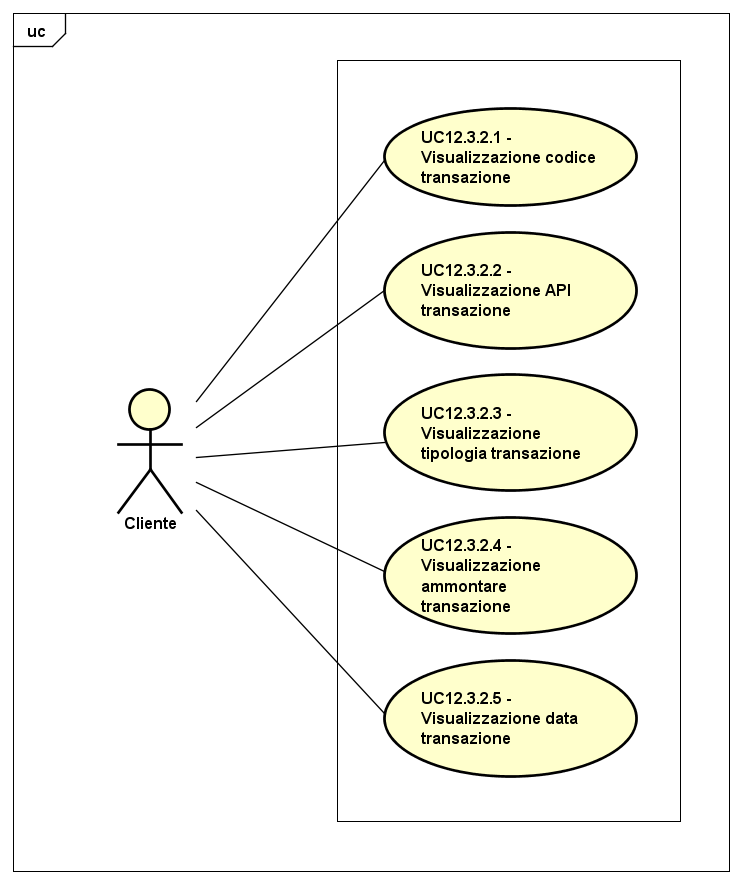
\includegraphics[scale=0.45]{UML/UC12_3_2.png}
	\caption{UC12.3.2: Visualizzazione lista transazioni concluse}
\end{figure}

\begin{minipage}{\linewidth}
	\begin{tabular}{ l | p{11cm}}
		\hline
		\rowcolor{Gray}
		\multicolumn{2}{c}{UC12.3.2 - Visualizzazione lista transazioni concluse} \\
		\hline
		\textbf{Attori} & Cliente \\
		\textbf{Descrizione} & L'attore visualizza la lista delle proprie transazioni \\
		\textbf{Pre-Condizioni} & L'attore si trova nella schermata relativa alla visualizzazione dello storico delle proprie transazioni \\
		\textbf{Post-Condizioni} & L'attore ha visualizzato la lista delle proprie transazioni \\
		\textbf{Scenario Principale} & 
		\begin{enumerate*}[label=(\arabic*.),itemjoin={\newline}]
			\item L'attore può visualizzare il codice della transazione (UC12.3.2.1)
			\item L'attore può visualizzare l'API di riferimento alla transazione (UC12.3.2.2)
			\item L'attore può visualizzare la tipologia della transazione (UC12.3.2.3)
			\item L'attore può visualizzare l'ammontare del denaro coinvolto nella transazione (UC12.3.2.4)
			\item L'attore può visualizzare la data della transazione (UC12.3.2.5)
		\end{enumerate*}\\
	\end{tabular}
\end{minipage}

\subparagraph{Caso d'uso UC12.3.2.1: Visualizzazione codice transazione}
\label{UC12_3_2_1}

\begin{minipage}{\linewidth}
	\begin{tabular}{ l | p{11cm}}
		\hline
		\rowcolor{Gray}
		\multicolumn{2}{c}{UC12.3.2.1 - Visualizzazione codice transazione} \\
		\hline
		\textbf{Attori} & Cliente \\
		\textbf{Descrizione} & L'attore visualizza il codice della propria transazione \\
	\textbf{Pre-Condizioni} & L'attore si trova nella schermata relativa alla visualizzazione dello storico delle proprie transazioni \\
	\textbf{Post-Condizioni} & L'attore ha visualizzato il codice della propria transazione \\
	\textbf{Scenario Principale} & 
	\begin{enumerate*}[label=(\arabic*.),itemjoin={\newline}]
		\item L'attore può visualizzare il codice della propria transazione
	\end{enumerate*}
	\end{tabular}
\end{minipage}

\subparagraph{Caso d'uso UC12.3.2.2: Visualizzazione API transazione}
\label{UC12_3_2_2}

\begin{minipage}{\linewidth}
	\begin{tabular}{ l | p{11cm}}
		\hline
		\rowcolor{Gray}
		\multicolumn{2}{c}{UC12.3.2.2 - Visualizzazione API transazione} \\
		\hline
		\textbf{Attori} & Cliente \\
		\textbf{Descrizione} & L'attore visualizza l'API di riferimento alla propria transazione \\
	\textbf{Pre-Condizioni} & L'attore si trova nella schermata relativa alla visualizzazione dello storico delle proprie transazioni \\
	\textbf{Post-Condizioni} & L'attore ha visualizzato l'API di riferimento alla propria transazione \\
	\textbf{Scenario Principale} & 
	\begin{enumerate*}[label=(\arabic*.),itemjoin={\newline}]
		\item L'attore può visualizzare l'API di riferimento alla propria transazione
	\end{enumerate*}
	\end{tabular}
\end{minipage}

\subparagraph{Caso d'uso UC12.3.2.3: Visualizzazione tipologia transazione}
\label{UC12_3_2_3}

\begin{minipage}{\linewidth}
	\begin{tabular}{ l | p{11cm}}
		\hline
		\rowcolor{Gray}
		\multicolumn{2}{c}{UC12.3.2.3 - Visualizzazione tipologia transazione} \\
		\hline
		\textbf{Attori} & Cliente \\
		\textbf{Descrizione} & L'attore visualizza la tipologia della propria transazione \\
	\textbf{Pre-Condizioni} & L'attore si trova nella schermata relativa alla visualizzazione dello storico delle proprie transazioni \\
	\textbf{Post-Condizioni} & L'attore ha visualizzato la tipologia della propria transazione \\
	\textbf{Scenario Principale} & 
	\begin{enumerate*}[label=(\arabic*.),itemjoin={\newline}]
		\item L'attore può visualizzare la tipologia della propria transazione
	\end{enumerate*}
	\end{tabular}
\end{minipage}

\subparagraph{Caso d'uso UC12.3.2.4: Visualizzazione ammontare transazione}
\label{UC12_3_2_4}

\begin{minipage}{\linewidth}
	\begin{tabular}{ l | p{11cm}}
		\hline
		\rowcolor{Gray}
		\multicolumn{2}{c}{UC12.3.2.4 - Visualizzazione ammontare transazione} \\
		\hline
		\textbf{Attori} & Cliente \\
		\textbf{Descrizione} & L'attore visualizza l'ammontare coinvolto nella propria transazione \\
	\textbf{Pre-Condizioni} & L'attore si trova nella schermata relativa alla visualizzazione dello storico delle proprie transazioni \\
	\textbf{Post-Condizioni} & L'attore ha visualizzato l'ammontare coinvolto nella propria transazione propria transazione \\
	\textbf{Scenario Principale} & 
	\begin{enumerate*}[label=(\arabic*.),itemjoin={\newline}]
		\item L'attore può visualizzare l'ammontare coinvolto nella propria transazione propria transazione
	\end{enumerate*}
	\end{tabular}
\end{minipage}

\subparagraph{Caso d'uso UC12.3.2.5: Visualizzazione data transazione}
\label{UC12_3_2_5}

\begin{minipage}{\linewidth}
	\begin{tabular}{ l | p{11cm}}
		\hline
		\rowcolor{Gray}
		\multicolumn{2}{c}{UC12.3.2.5 - Visualizzazione data transazione} \\
		\hline
		\textbf{Attori} & Cliente \\
		\textbf{Descrizione} & L'attore visualizza la data della propria transazione \\
	\textbf{Pre-Condizioni} & L'attore si trova nella schermata relativa alla visualizzazione dello storico delle proprie transazioni \\
	\textbf{Post-Condizioni} & L'attore ha visualizzato la data della propria transazione \\
	\textbf{Scenario Principale} & 
	\begin{enumerate*}[label=(\arabic*.),itemjoin={\newline}]
		\item L'attore può visualizzare la data della propria transazione
	\end{enumerate*}
	\end{tabular}
\end{minipage}

\newpage
\paragraph{Caso d'uso UC12.3.3: Visualizzazione lista credito}
\label{UC12_3_3}
\begin{figure}[ht]
	\centering
	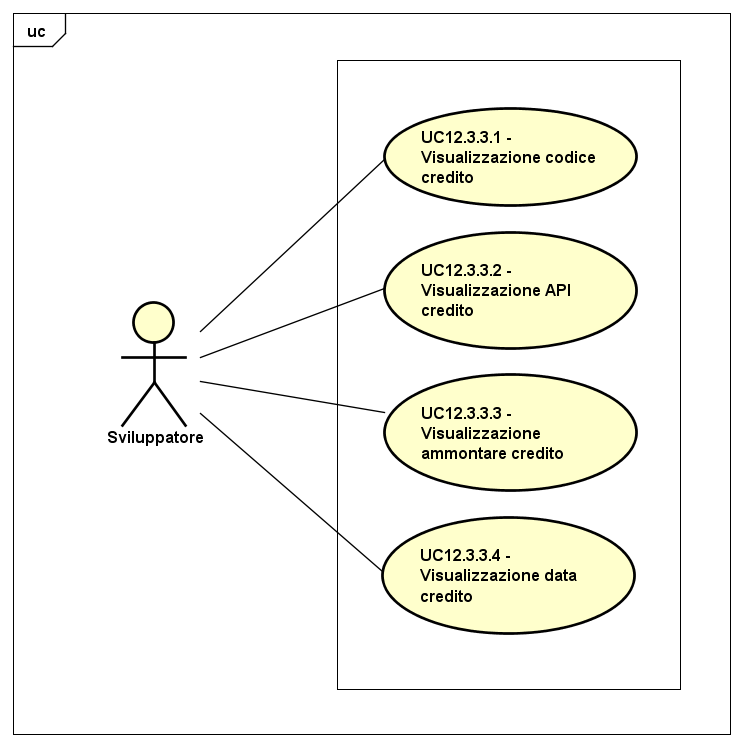
\includegraphics[scale=0.45]{UML/UC12_3_3.png}
	\caption{UC12.3.3: Visualizzazione lista credito}
\end{figure}

\begin{minipage}{\linewidth}
	\begin{tabular}{ l | p{11cm}}
		\hline
		\rowcolor{Gray}
		\multicolumn{2}{c}{UC12.3.3 - Visualizzazione lista credito} \\
		\hline
		\textbf{Attori} & Sviluppatore \\
		\textbf{Descrizione} & L'attore visualizza la lista dei propri crediti \\
		\textbf{Pre-Condizioni} & L'attore si trova nella schermata relativa alla visualizzazione dello storico delle proprie transazioni \\
		\textbf{Post-Condizioni} & L'attore ha visualizzato la lista dei propri crediti \\
		\textbf{Scenario Principale} & 
		\begin{enumerate*}[label=(\arabic*.),itemjoin={\newline}]
			\item L'attore può visualizzare il codice del credito (UC12.3.3.1)
			\item L'attore può visualizzare l'API di riferimento al credito (UC12.3.3.2)
			\item L'attore può visualizzare l'ammontare del credito accumulato per l'API di riferimento (UC12.3.3.3)
			\item L'attore può visualizzare la data del credito (UC12.3.3.4)
		\end{enumerate*}\\
	\end{tabular}
\end{minipage}

\subparagraph{Caso d'uso UC12.3.3.1: Visualizzazione codice credito}
\label{UC12_3_3_1}

\begin{minipage}{\linewidth}
	\begin{tabular}{ l | p{11cm}}
		\hline
		\rowcolor{Gray}
		\multicolumn{2}{c}{UC12.3.3.1 - Visualizzazione codice credito} \\
		\hline
		\textbf{Attori} & Sviluppatore \\
		\textbf{Descrizione} & L'attore visualizza il codice del proprio credito \\
	\textbf{Pre-Condizioni} & L'attore si trova nella schermata relativa alla visualizzazione dello storico delle proprie transazioni \\
	\textbf{Post-Condizioni} & L'attore ha visualizzato il codice del proprio credito \\
	\textbf{Scenario Principale} & 
	\begin{enumerate*}[label=(\arabic*.),itemjoin={\newline}]
		\item L'attore può visualizzare il codice del proprio credito
	\end{enumerate*}
	\end{tabular}
\end{minipage}

\subparagraph{Caso d'uso UC12.3.3.2: Visualizzazione API credito}
\label{UC12_3_3_2}

\begin{minipage}{\linewidth}
	\begin{tabular}{ l | p{11cm}}
		\hline
		\rowcolor{Gray}
		\multicolumn{2}{c}{UC12.3.3.2 - Visualizzazione API credito} \\
		\hline
		\textbf{Attori} & Sviluppatore \\
		\textbf{Descrizione} & L'attore visualizza l'API di riferimento al proprio credito \\
	\textbf{Pre-Condizioni} & L'attore si trova nella schermata relativa alla visualizzazione dello storico delle proprie transazioni \\
	\textbf{Post-Condizioni} & L'attore ha visualizzato l'API di riferimento al proprio credito \\
	\textbf{Scenario Principale} & 
	\begin{enumerate*}[label=(\arabic*.),itemjoin={\newline}]
		\item L'attore può visualizzare l'API di riferimento al proprio credito
	\end{enumerate*}
	\end{tabular}
\end{minipage}
	
\subparagraph{Caso d'uso UC12.3.3.3: Visualizzazione ammontare credito}
\label{UC12_3_3_3}

\begin{minipage}{\linewidth}
	\begin{tabular}{ l | p{11cm}}
		\hline
		\rowcolor{Gray}
		\multicolumn{2}{c}{UC12.3.3.3 - Visualizzazione ammontare credito} \\
		\hline
		\textbf{Attori} & Sviluppatore \\
		\textbf{Descrizione} & L'attore visualizza l'ammontare del proprio credito per l'API di riferimento \\
	\textbf{Pre-Condizioni} & L'attore si trova nella schermata relativa alla visualizzazione dello storico delle proprie transazioni \\
	\textbf{Post-Condizioni} & L'attore ha visualizzato ll'ammontare del proprio credito per l'API di riferimento \\
	\textbf{Scenario Principale} & 
	\begin{enumerate*}[label=(\arabic*.),itemjoin={\newline}]
		\item L'attore può visualizzare l'ammontare del proprio credito per l'API di riferimento
	\end{enumerate*}
	\end{tabular}
\end{minipage}

\subparagraph{Caso d'uso UC12.3.3.4: Visualizzazione data credito}
\label{UC12_3_3_4}

\begin{minipage}{\linewidth}
	\begin{tabular}{ l | p{11cm}}
		\hline
		\rowcolor{Gray}
		\multicolumn{2}{c}{UC12.3.3.4 - Visualizzazione data credito} \\
		\hline
		\textbf{Attori} & Sviluppatore \\
		\textbf{Descrizione} & L'attore visualizza la data del proprio credito per l'API di riferimento \\
	\textbf{Pre-Condizioni} & L'attore si trova nella schermata relativa alla visualizzazione dello storico delle proprie transazioni \\
	\textbf{Post-Condizioni} & L'attore ha visualizzato la data del proprio credito per l'API di riferimento \\
	\textbf{Scenario Principale} & 
	\begin{enumerate*}[label=(\arabic*.),itemjoin={\newline}]
		\item L'attore può visualizzare la data del proprio credito per l'API di riferimento
	\end{enumerate*}
	\end{tabular}
\end{minipage}